\documentclass{article}
\usepackage{graphicx}
\usepackage[utf8]{inputenc}

\title{
{Tech Review } \\
{\large VR Training Program For HP's PageWide Web Press} \\
{\small Group 73}
\author{Stewart Rodger }
}
\date{November 2018}
\begin{document}

\maketitle

\section*{Abstract}
Virtual Reality shows considerable promise in cutting costs and speeding up training for large machinery like the Page-Wide Web Press. By using a virtual training program, companies can drastically shorten the in person training. Our team will develop a series of virtual training programs for HPs PageWide Web Press product line designed to achieve these goals. In order to achieve this we must have a strong grasp on the the various perspectives and data collection methods necessary to ensure a maximally effective training simulation.      

\section{Game/Simulation Perspective}
In any game or simulation, there are 3 primary camera positions. "First Person" places the camera on the controlled object or avatar, showing things at eye level. "Third Person" positions the camera behind and slightly above the controlled character. "Overhead" is a camera that is placed high above the scene or level, pointed down. In the image below, A is overhead, B is 1st person, and C and D are 3rd person. [1] 

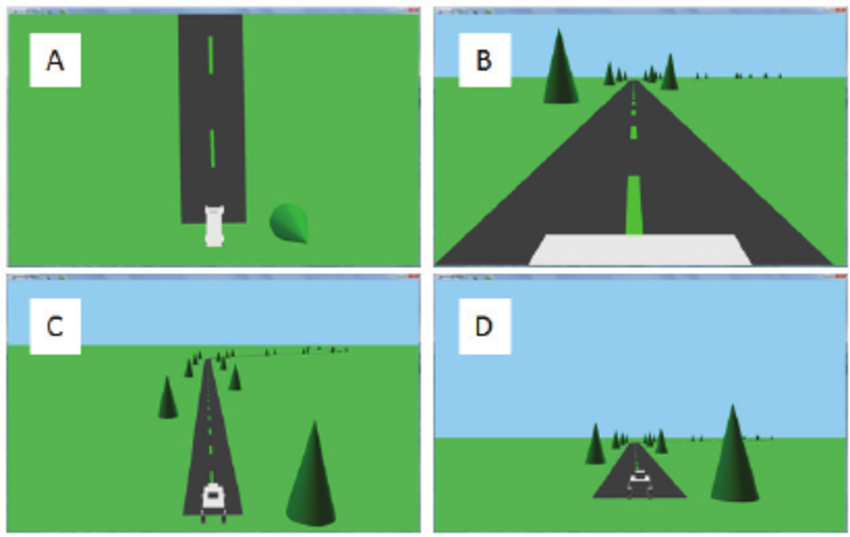
\includegraphics[width=\textwidth]{13o.png}

It is commonly known in game development that the choice of perspective is important to the overall design and "failure to take this particular gameplay element seriously will very likely result in your game controlling horribly, and having a disjointed 'feel'"[2]. Focusing on the camera's value for simulations, there are a few distinct benefits for each option. 

\subsection{Overhead View}
The overhead view provides a complete view of the scene without having to move the camera. This can simplify the control scheme as the user does not need to worry about controlling the view. The other main benefit of this view is that the user can see everything in the room or scene at once. This allows the user to see cause and effect when interacting with objects that have effects that might be out of view with other camera angles. The downsides is that this is the most dissociative of the camera angles. With overhead view is actions feel the least real, and for complex situations the camera may need to change as it is unable to show the side of a object or machine in detail.

\subsection{3rd Person View}
The 3rd person camera is the middle ground option. The 3rd person camera still provides a larger field of view than 1st person, while showing the simulation in a more realistic was as the camera is closer to eye level and can properly show the sides of objects. Unfortunately, the 3rd person camera requires the most input controls of the three, and it also is still less immersive than 1st person because the 3rd person allows you to see the back of the avatar being controlled.  

\subsection{1st Person View}
1st person camera angle is the most immersive of the three [2], with the camera simulating the actual field of view for the controlled character. The downside of first person view is that the the controls can be the most disorienting for users who are inexperienced with virtual environments. First person has a distinct advantage in one area, It is uniquely compatible with a Virtual Reality (VR) headset and control scheme. VR generally does not make 3rd person or Overhead camera controls more convenient or simpler, however it provides both of these benefits to first person view. 


\section{Data Collection}
An important part of any training simulation is the collection of data. The right kinds of data, collected periodically throughout the test runs, can show what parts of a simulation are flawed, or what parts of the training require more explanation or instruction. However, do to the costs of implementation, "evaluators should focus more on what are those important aspects in game experience (like playability) that we should measure in order to be able to evaluate the game properly, and then select the tools that meet those requirements." [3] There are a few different ways to go about saving user data, the most beneficial are Success/failure counting and Time counting, however there also is an extreme form of data collection through interaction counting.

\subsection{Success/Failure counting}
Success/Failure counting involves having a system in place to count the number of times a user fails for each task they are attempting to complete. Every time a user, preferably a new test user, is run though the training program, the success/failure count is collected so that we can see what sections were the most prone to errors. The number of failures should be lowered as much as possible though the addition of new objective markers, more or clearer instructions, and the reevaluation of the program to ensure that the success/failure rate is improving. An important aspect of success/failure counting is what to count as an objective worthy of counting the failures for. This results in 2 different methods for success/failure counting, "Basic" and "Hidden".

\subsubsection{Basic success/failure}
"Basic" success/failure counting only counts the failure if the user fails to properly complete a objective that they know is a clear objective. For example, if they are provided with a list of tasks to complete, the system will only count if they have failed or completed those tasks. This is the most basic form of failure counting, and it can provide a lot of valuable data about the tasks and the quality of the instructions or simulation. In addition it is relatively quick and cheap to implement. The downsides are that it may miss valuable data by being limited in scope. That is where "hidden" success/failure counting comes in.

\subsubsection{Hidden success/failure}
 "Hidden" success/failure counting works as an extension of "Basic" counting.  Instead of counting just the clear objectives, you also have a number of objectives that are not displayed (for example: Did the user interact with the objects in the ideal order, even if that order was not required to succeed?). This provides substantially more data at the cost of development time, as there is no simple list of things to do like with "Basic" counting. This method also cost time later as the data it provides will take more time to sort through. 

\subsection{Time Counting}
The 2nd main form of data collection is time counting. With this form of data collection the system starts and runs a number of stopwatches in the background and saves the results for specific tasks. A timer begins when the user starts a task and saves when they complete it. The extent of this varies directly with the amount of data the developer is willing to collect and sort through. 


\subsubsection{Count total time}
Just like with success/failure, time counting can be applied in a limited capacity, focusing on only the main objectives. In this case the developer can track time from training program launch to success, and track the individual objective attempt times, while keeping development costs/time low. 


\subsubsection{Count time between specific actions}
Also similar to success/failure, time counting can be applied to an ever expanding quantity of other hidden objectives. An example could be tracking the time a user spends from when they start the training program to when they first move to learn if they are taking a long time interpreting the instructions.


\subsection{Interaction Counting}
Interaction counting is exactly how it sounds in the context of the previous two methods. Systems are put in place in the background of the simulation to count every time the user interacts with a specific object or objects. The number of objects that are being watched can vary from 1 to every interact-able object, and clicking on the screen. It is directly expandable to meet the time and cost constraints of development, and it can provide data that the previous methods might miss. Unfortunately, this comes at the cost of a greatly increased data interpretation time. One of the greatest benefits of this method is less about improving user interaction and more about bug fixing. With this method in place, assuming a large enough percentage of objects being tracked, it is possible to recreate the users inputs to find the specific series of events that caused a bug or error to occur. 


\section*{Conclusion}
For the purposes of this VR training program, 1st person view is the obvious choice. VR will help negate the extra control complications, while providing the most immersive simulation experience we can deliver. For data collection, We will want to use basic form of success/failure and time counting. This will get us the most viable user data while minimizing the amount of extra development time or data analysis time. 

\newpage
\section*{References}
[1] https://www.researchgate.net/figure/The-four-views-A-overhead-B-first-person-C-third-person-high-D-third-person-low\_fig1\_221474898
\break
[2]  https://www.gamasutra.com/blogs/MichelSabbagh/20150827/252341/The\_important\_differences\_between\_firstperson\_and\_thirdperson\_games.php
\break
[3]  http://tampub.uta.fi/bitstream/handle/10024/79391/gradu03017.pdf;sequence=1

\end{document}
